% Rolling out-of-sample design (bgarch_experiments.walkforward): refit every 63 trading days on the last
% W = 500 or 1000 returns; between refits parameters are frozen and the variance is filtered daily.
\documentclass[tikz,border=3pt]{standalone}
% Shared look for the narrative diagrams (included by portfolio_flowchart.tex and rolling_design.tex)
\usepackage[T1]{fontenc}
\usepackage{lmodern}
\usepackage{amsmath,amssymb}
\renewcommand{\familydefault}{\sfdefault}
\usetikzlibrary{positioning,arrows.meta,calc,fit,backgrounds,decorations.pathreplacing}
\definecolor{ink}{HTML}{1F1F1E}
\definecolor{muted}{HTML}{6B6A63}
\definecolor{fc}{HTML}{2A78D6}   % statistical forecasting
\definecolor{al}{HTML}{EB6834}   % portfolio allocation
\definecolor{ex}{HTML}{1BAF7A}   % execution and accounting
\definecolor{ev}{HTML}{7A5BB5}   % performance evaluation
\definecolor{rule}{HTML}{D9D7CF}
\tikzset{
  box/.style={draw=#1, fill=#1!9, line width=0.8pt, rounded corners=3pt, align=flush left,
              inner sep=3.2pt, text=ink, font=\small},
  step/.style={box=#1, text width=3.75cm, minimum height=1.45cm},
  arr/.style={-{Stealth[length=2.4mm]}, line width=0.9pt, draw=muted},
  num/.style={circle, fill=#1, text=white, font=\scriptsize\bfseries, inner sep=1.2pt, minimum size=4mm},
}

\begin{document}
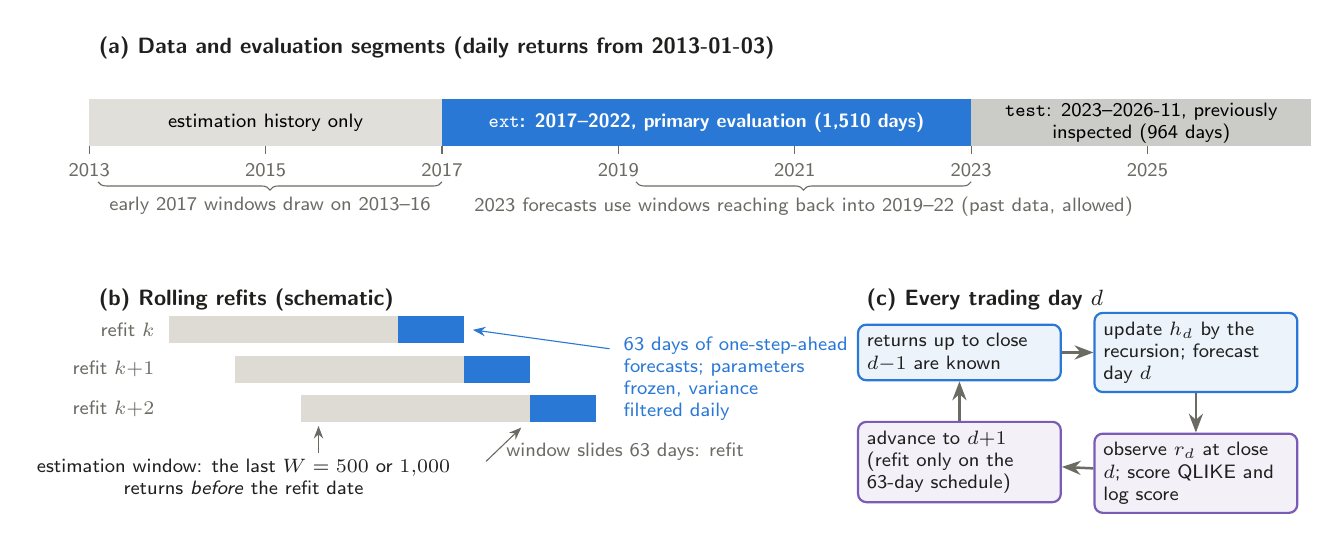
\begin{tikzpicture}[x=1.12cm,y=1cm]
% ---------------- (a) calendar of the data
\node[anchor=west, font=\footnotesize\bfseries, text=ink] at (0,1.25) {(a) Data and evaluation segments (daily returns from 2013-01-03)};
\fill[rule!80] (0,0) rectangle (4,0.6);
\fill[fc] (4,0) rectangle (10,0.6);
\fill[muted!35] (10,0) rectangle (13.85,0.6);
\node[font=\scriptsize, align=center] at (2,0.3) {estimation history only};
\node[font=\scriptsize\bfseries, text=white, align=center] at (7,0.3) {\texttt{ext}: 2017--2022, primary evaluation (1{,}510 days)};
\node[font=\scriptsize, align=center] at (11.93,0.3) {\texttt{test}: 2023--2026-11, previously\\inspected (964 days)};
\foreach \x/\l in {0/2013,2/2015,4/2017,6/2019,8/2021,10/2023,12/2025} {\draw[muted] (\x,0)--(\x,-0.1) node[below,font=\scriptsize,text=muted]{\l};}
\draw[decorate,decoration={brace,amplitude=3pt,mirror},muted] (6.2,-0.45)--(10,-0.45)
   node[midway,below=2pt,font=\scriptsize,text=muted,align=center] {2023 forecasts use windows reaching back into 2019--22 (past data, allowed)};
\draw[decorate,decoration={brace,amplitude=3pt,mirror},muted] (0.1,-0.45)--(4,-0.45)
   node[midway,below=2pt,font=\scriptsize,text=muted,align=center] {early 2017 windows draw on 2013--16};
% ---------------- (b) rolling refits (schematic, not to scale)
\begin{scope}[yshift=-1.95cm]
\node[anchor=west, font=\footnotesize\bfseries, text=ink] at (0,0) {(b) Rolling refits (schematic)};
\foreach \k/\lab in {0/{refit $k$},1/{refit $k{+}1$},2/{refit $k{+}2$}} {
  \pgfmathsetmacro{\y}{-0.55-0.5*\k}
  \pgfmathsetmacro{\a}{0.9+0.75*\k}
  \fill[rule!90] (\a,\y) rectangle ++(2.6,0.34);
  \fill[fc] (\a+2.6,\y) rectangle ++(0.75,0.34);
  \node[font=\scriptsize, anchor=east, text=muted] at (0.85,\y+0.17) {\lab};
}
\node[font=\scriptsize] at (2.5,-0.38) {};
\node[font=\scriptsize, align=center, text=ink] at (1.75,-2.25) {estimation window: the last $W=500$ or $1{,}000$\\returns \emph{before} the refit date};
\draw[muted,-{Stealth[length=1.6mm]}] (2.6,-1.95)--(2.6,-1.6);
\node[font=\scriptsize, align=left, text=fc, anchor=west] at (5.95,-1.0) {63 days of one-step-ahead\\forecasts; parameters\\frozen, variance\\filtered daily};
\draw[fc,-{Stealth[length=1.6mm]}] (5.9,-0.62)--(4.35,-0.38);
\draw[muted,-{Stealth[length=1.6mm]}] (4.5,-2.05) -- node[right,font=\scriptsize,text=muted,pos=.3]{window slides 63 days: refit} (4.9,-1.62);
\end{scope}
% ---------------- (c) daily loop
\begin{scope}[xshift=9.75cm,yshift=-1.95cm]
\node[anchor=west, font=\footnotesize\bfseries, text=ink] at (0,0) {(c) Every trading day $d$};
\node[box=fc, text width=2.35cm, font=\scriptsize, anchor=north west] (d1) at (0,-0.3) {returns up to close $d{-}1$ are known};
\node[box=fc, text width=2.35cm, font=\scriptsize, right=4mm of d1] (d2) {update $h_d$ by the recursion; forecast day $d$};
\node[box=ev, text width=2.35cm, font=\scriptsize, below=5mm of d2] (d3) {observe $r_d$ at close $d$; score QLIKE and log score};
\node[box=ev, text width=2.35cm, font=\scriptsize, below=5mm of d1] (d4) {advance to $d{+}1$ (refit only on the 63-day schedule)};
\draw[arr] (d1)--(d2); \draw[arr] (d2)--(d3); \draw[arr] (d3)--(d4); \draw[arr] (d4)--(d1);
\end{scope}
\end{tikzpicture}
\end{document}
